\documentclass[conference]{IEEEtran}
\IEEEoverridecommandlockouts
\usepackage{cite}
\usepackage{amsmath,amssymb}
\usepackage{bm}
\usepackage{graphicx}
\usepackage{booktabs}
\usepackage{siunitx}
\usepackage{tikz}
\usetikzlibrary{arrows.meta,positioning,fit,backgrounds,calc}
\usepackage[hidelinks]{hyperref}
\sisetup{detect-all, per-mode=symbol, range-phrase=--, range-units=single}
\newcommand{\T}{^{\mathsf T}}
\newcommand{\half}{\tfrac{1}{2}}
\graphicspath{{figs/}}

\begin{document}

\title{Observer-Based Digital Ride-Height Control of a\\ Fully Submerged Hydrofoil Boat}

\author{\IEEEauthorblockN{Shengwei Li and Hengfei Xu}
\IEEEauthorblockA{\textit{School of Electrical and Computer Engineering} \\
\textit{The University of Sydney}, NSW, Australia}}

\maketitle

\begin{abstract}
Fully submerged hydrofoils give a small boat low drag and a smooth ride, but
their lift hardly depends on depth, so the boat cannot hold a ride height
without feedback. We model the heave and pitch dynamics of a solar-powered
hydrofoil boat from first principles, with parameters of the T\'ecnico Solar
Boat SR02, including the loss of lift near the free surface, actuator limits,
sensor noise and irregular head seas. Linearised at cruise speed, the plant is
unstable and has four states but only three sensors, and the height sensor sees
the water surface as well as the boat. We design a digital controller running
at 50 Hz that combines linear quadratic state feedback with integral action and
a Kalman filter with a force-bias state, and compare the filter with
pole-placement observers. On the nonlinear model the controller settles a 5 cm
height step in 2.2 s without overshoot, holds the height within 1 cm rms in
regular waves and removes the steady-state error caused by speed and mass
errors. Run as a separate real-time process connected to the simulated boat
over a network link, the same controller reproduces these results exactly and
tolerates replies one sample late.
\end{abstract}

\begin{IEEEkeywords}
hydrofoil, ride-height control, LQR, Kalman filter, digital control,
software in the loop
\end{IEEEkeywords}

%=====================================================================
\section{Introduction}

A hydrofoil lifts the hull out of the water and cuts its drag at speed, which
matters most for boats with little power, such as the solar boats of student
competitions \cite{belime,marrewijk}. Surface-piercing foils
regulate their own depth because their wetted span changes with height. Fully
submerged foils are disturbed less by waves, but their lift is almost
independent of depth \cite{faltinsen}; a boat carried by them has almost no ride-height
stiffness and must be stabilised by changing the foil incidence
\cite{faltinsen,belime}.

Belime \cite{belime} modelled the SR02 boat of the T\'ecnico Solar Boat team,
designed an LQR with integral action at \SI{7}{m/s} and flew it. In the trials
the boat accelerated after take-off and left the speed the controller was
designed for, so a separate speed loop on the motors was added; gain scheduling
and an actuated rear foil were left as future work. Van Marrewijk and
Schonebaum \cite{marrewijk} derived and experimentally validated a dynamic model
of a single-track hydrofoil boat. For larger craft, Ren and Yang \cite{renyang}
replaced a single LQR by fuzzy gain scheduling over the operating range of a
hydrofoil catamaran, and Liu et~al.\ \cite{liu} combined LQR output regulation
with sliding-mode control to reduce the heave and pitch of a fully submerged
hydrofoil craft in waves.

The single-point design of \cite{belime} is simple and has flown, but it is
sensitive to speed. Gain scheduling \cite{renyang} covers the speed range at the
cost of a fuzzy model and an LMI stability test, and the sliding-mode design of
\cite{liu} adds robustness, with weights tuned by a genetic algorithm, and was
evaluated in simulation. On a small boat a further difficulty is the measurement: the
ride height comes from a single ultrasonic sensor at the bow, which measures the
distance to the water surface, not the height of the boat above its mean level.
This paper treats that problem explicitly within the observer-based state
feedback framework. Its
contributions are:
\begin{enumerate}
\item a first-principles nonlinear heave and pitch model with free-surface
      effect and wave disturbances, checked against the trim of \cite{belime};
\item an observer-based controller in which a Kalman filter with a force-bias
      state separates the boat motion from the water surface, compared with
      pole-placement observers;
\item a direct digital design at \SI{50}{Hz} with a computation delay, tested on
      the nonlinear model in regular and irregular seas and under model error;
\item a software-in-the-loop test in which the controller runs as a separate
      real-time process, which measures how late its commands may be.
\end{enumerate}
Section~\ref{sec:model} develops the model, Section~\ref{sec:problem} defines
the control problem and the design criteria, Section~\ref{sec:design} designs
the controller and observer, Section~\ref{sec:valid} validates them in
simulation, and Section~\ref{sec:concl} concludes.

%=====================================================================
\section{System Model}
\label{sec:model}

\subsection{Boat and assumptions}

SR02 is a single-seat solar boat of \SI{215}{kg} with pilot \cite{belime}. Two
front foils, moved together, and one rear foil on the propulsion strut carry
it when foil-borne (Fig.~\ref{fig:boat}). The control inputs are the incidence
angles $\delta_f$, $\delta_r$ of the front and rear foils relative to the hull.
We assume:
(A1) the hull is clear of the water;
(A2) the motion is in the vertical plane (heave and pitch);
(A3) the forward speed $U$ is constant, being held by a separate speed loop
\cite{belime}; deviations are treated as model uncertainty;
(A4) foil drag and thrust are neglected in the heave and pitch equations (their
net moment is about \SI{1}{\percent} of the foil moments);
(A5) lift is quasi-steady and affine in the angle of attack below stall
(\SI{12}{\degree});
(A6) the added mass of the foils is neglected (\SI{4}{\percent} of the mass);
(A7) the rear foil is actuated, which \cite{belime} lists as future work.

\begin{figure}[t]
\centering
% Side view of the boat (schematic, lengths in metres, body axes at trim)
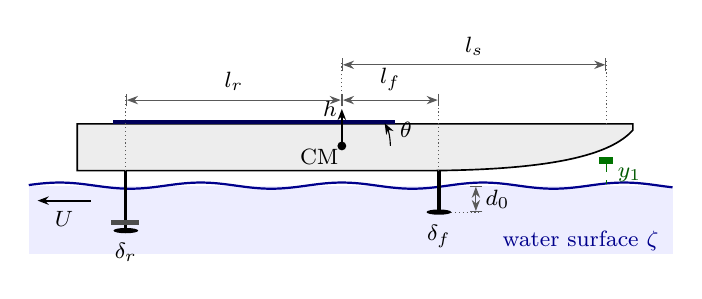
\begin{tikzpicture}[x=1.12cm, y=1.12cm, >={Stealth[length=4pt]}, font=\footnotesize]
  % water
  \fill[blue!7] (-3.55,-1.22) rectangle (3.75,-0.45);
  \draw[blue!55!black, thick, domain=-3.55:3.75, samples=120, smooth]
       plot (\x, {-0.45 + 0.035*cos(deg(2*pi*\x/1.6))});
  \node[blue!55!black, anchor=east] at (3.7,-1.08) {water surface $\zeta$};
  % hull
  \filldraw[fill=gray!14, draw=black, line width=0.6pt]
    (-3.0,-0.28) -- (1.0,-0.28) .. controls (2.4,-0.27) and (3.05,-0.10) .. (3.3,0.18)
    -- (3.3,0.25) -- (-3.0,0.25) -- cycle;
  \fill[blue!35!black] (-2.6,0.25) rectangle (0.6,0.29);
  % struts and foils
  \draw[line width=1.2pt] (1.10,-0.28) -- (1.10,-0.75);
  \draw[line width=1.2pt] (-2.45,-0.28) -- (-2.45,-0.96);
  \fill (1.10,-0.75) ellipse (0.14 and 0.03);
  \fill (-2.45,-0.96) ellipse (0.14 and 0.03);
  \fill[gray!60!black] (-2.62,-0.90) rectangle (-2.30,-0.84);
  \node[anchor=north] at (1.10,-0.79) {$\delta_f$};
  \node[anchor=north] at (-2.45,-0.99) {$\delta_r$};
  % centre of mass and states
  \fill (0,0) circle (1.6pt);
  \node[anchor=north east, inner sep=1pt] at (0,0) {CM};
  \draw[->, thick] (0,0) -- (0,0.42) node[anchor=east, inner sep=1.5pt] {$h$};
  \draw[->] (0.55,0) arc[start angle=0, end angle=28, radius=0.55];
  \node[anchor=west] at (0.55,0.18) {$\theta$};
  % sensor and beam
  \fill[green!45!black] (2.92,-0.20) rectangle (3.08,-0.12);
  \draw[green!45!black, dashed] (3.0,-0.20) -- (3.0,-0.43);
  \node[green!35!black, anchor=west] at (3.02,-0.33) {$y_1$};
  % dimensions
  \draw[|<->|, gray!70!black] (0,0.52) -- node[above, black] {$l_f$} (1.10,0.52);
  \draw[|<->|, gray!70!black] (-2.45,0.52) -- node[above, black] {$l_r$} (0,0.52);
  \draw[|<->|, gray!70!black] (0,0.92) -- node[above, black] {$l_s$} (3.0,0.92);
  \draw[gray!70!black, densely dotted] (0,0.45) -- (0,0.97);
  \draw[gray!70!black, densely dotted] (1.10,-0.28) -- (1.10,0.57) (-2.45,-0.28) -- (-2.45,0.57) (3.0,0.25) -- (3.0,0.97);
  \draw[|<->|, gray!70!black] (1.52,-0.45) -- node[right, black] {$d_0$} (1.52,-0.75);
  \draw[gray!70!black, densely dotted] (1.24,-0.75) -- (1.58,-0.75);
  % flow
  \draw[<-, thick] (-3.45,-0.62) -- node[below] {$U$} (-2.85,-0.62);
\end{tikzpicture}

\caption{Side view of the boat in body axes at trim: centre of mass (CM),
front and rear foils, bow height sensor and the states $h$, $\theta$.}
\label{fig:boat}
\end{figure}

\subsection{Equations of motion}

The state is $\bm x=[\,h\;\;v\;\;\theta\;\;q\,]\T$: heave of the CM (up
positive), its rate, pitch (bow up positive) and pitch rate. Foil
$i\in\{f,r\}$ lies $x_i$ ahead of and $z_i$ below the CM. Its velocity relative
to the water is
\begin{equation}
u_i=U+q\,(z_i\cos\theta-x_i\sin\theta),\quad
v_i=v+q\,X_i-w_i,
\label{eq:vfoil}
\end{equation}
where $X_i=x_i\cos\theta+z_i\sin\theta$ and $w_i$ is the vertical water
velocity from waves. The inflow angle $\gamma_i=\arctan(v_i/u_i)$ reduces the
angle of attack, $\alpha_i=\delta_i+\theta-\gamma_i$, which damps heave and
pitch. The lift is
\begin{equation}
L_i=\half\rho\,(u_i^2+v_i^2)\,S_i\,K(d_i/c)\,(C_{L0}+C_{L\alpha}\alpha_i),
\label{eq:lift}
\end{equation}
with submergence $d_i=d_0-h-x_i\sin\theta-z_i(1-\cos\theta)$ and the
free-surface factor of linear foil theory at high Froude number
($U/\sqrt{gd_0}\approx4.1$) \cite{faltinsen},
\begin{equation}
K(\xi)=\frac{1+16\xi^2}{2+16\xi^2},\qquad \xi=d/c ,
\label{eq:K}
\end{equation}
which falls from 1 deep down to $\half$ at the surface; in simulation $K=0$ once
a foil leaves the water. With $Z_i=x_i\sin\theta-z_i\cos\theta$, Newton's laws
give
\begin{align}
m\dot v &= \textstyle\sum_i L_i\cos\gamma_i-mg, \label{eq:heave}\\
I_y\dot q &= \textstyle\sum_i L_i\,(X_i\cos\gamma_i+Z_i\sin\gamma_i),
\label{eq:pitch}
\end{align}
with $\dot h=v$, $\dot\theta=q$. The nonlinearities are the trigonometric
terms, the velocity-squared dynamic pressure, $K$, stall and the actuator
limits.

\subsection{Actuators, sensors and waves}

The foil actuators have an absolute range of \SI{-3}{\degree} to
\SI{7}{\degree} \cite{belime}; we assume a rate limit of \SI{20}{\degree/s} and,
in simulation, a first-order servo lag of \SI{20}{ms}. Encoders report the
actual foil angles. The sensors, as fitted to SR02 \cite{belime}, are an
ultrasonic height sensor $l_s$ ahead of the CM and an attitude reference unit
(AHRS) giving pitch and pitch rate; we assume all are sampled at \SI{50}{Hz}:
\begin{equation}
y_1=h+l_s\sin\theta-\zeta(l_s,t)+n_1,\quad y_2=\theta+n_2,\quad y_3=q+n_3,
\label{eq:meas}
\end{equation}
with white noise of standard deviation \SI{1}{cm}, \SI{0.3}{\degree} and
\SI{0.2}{\degree/s} (assumed). The term $\zeta$ is the water surface under the
sensor, which the height reading cannot distinguish from boat motion.

Waves are modelled by linear (Airy) theory in head seas as a sum of components,
\begin{align}
\zeta(x,t)&=\textstyle\sum_j a_j\cos(k_jx+\omega_{ej}t+\phi_j),\\
w_i(t)&=-\textstyle\sum_j a_j\omega_j e^{-k_jd_0}\sin(k_jx_i+\omega_{ej}t+\phi_j),
\end{align}
with $k_j=\omega_j^2/g$ and encounter frequency $\omega_{ej}=\omega_j+k_jU$. The
regular test wave has \SI{5}{cm} amplitude and \SI{8}{m} wavelength
($\omega_e=\SI{8.27}{rad/s}$, $w$ amplitude \SI{0.11}{m/s}). Irregular seas use
80 components of a JONSWAP spectrum ($\gamma=3.3$) \cite{jonswap} with random
phases.

\subsection{Parameters, limitations and uncertainty}

Table~\ref{tab:params} lists the parameters. The chord follows from the lift
slope and aspect-ratio correction of \cite{belime}; the submergence and the
noise levels are assumed. The model is valid foil-borne, near level flight; it
omits take-off, surge, unsteady lift, downwash of the front foils on the rear
foil, ventilation and the horizontal orbital velocity (about \SI{3}{\percent}
of dynamic pressure in the test wave). The main uncertainties are the speed,
which scales the control effectiveness with $U^2$, and the mass.

\begin{table}[t]
\centering
\caption{Model parameters (B: from \cite{belime}; E: estimated or assumed)}
\label{tab:params}
\small
\begin{tabular}{@{}lll@{\hspace{1.2em}}lll@{}}
\toprule
$m$ & \SI{215}{kg} & B & $C_{L0}$ & 0.288 & B \\
$I_y$ & \SI{503}{kg.m^2} & B & $C_{L\alpha}$ & \SI{5.16}{rad^{-1}} & B \\
$S_f,S_r$ & 0.096, \SI{0.046}{m^2} & B & $U_0$ & \SI{7}{m/s} & B \\
$x_f,x_r$ & 1.10, \SI{-2.45}{m} & B & $c$ & \SI{0.073}{m} & E \\
$z_f,z_r$ & 0.75, \SI{0.96}{m} & B & $d_0$ & \SI{0.30}{m} & E \\
$l_s$ & \SI{3.0}{m} & B & $\rho$ & \SI{1025}{kg/m^3} & B \\
\bottomrule
\end{tabular}
\end{table}

%=====================================================================
\section{Problem Definition}
\label{sec:problem}

\subsection{Control aims and operating point}

Without control the boat cannot hold a height (Section~\ref{sec:lin}). The
height must stay inside a narrow window: a foil that comes too close to the
surface loses lift and may ventilate, and a hull that drops by more than its
clearance of about \SI{0.3}{m} hits the water. The hull should also stay level,
for the pilot and to keep both foils near their design angle of attack. The
controller acts on $\delta_f,\delta_r$ and measures $y_1,y_2,y_3$ and the
encoders. It must reject waves, follow height commands from the pilot and cope
with speed and mass changes.

The operating point is level flight at the endurance speed $U_0=\SI{7}{m/s}$
\cite{belime} with the foils \SI{0.30}{m} deep. Setting
$\dot v=\dot q=0$ in \eqref{eq:heave}--\eqref{eq:pitch} shares the weight in
inverse proportion to the lever arms, $L_{f0}=\SI{1456}{N}$,
$L_{r0}=\SI{654}{N}$, and inverting \eqref{eq:lift} gives the trim incidences
$\delta_{f0}=\SI{3.53}{\degree}$, $\delta_{r0}=\SI{3.11}{\degree}$. These agree
with the numerical trim of \cite{belime}, which includes drag and thrust, to
within \SI{0.1}{\degree} from 6 to \SI{10}{m/s} (Table~\ref{tab:trim}),
supporting (A4).

\begin{table}[t]
\centering
\caption{Trim incidences (deg): this model and \cite{belime}}
\label{tab:trim}
\small
\begin{tabular}{@{}lccccc@{}}
\toprule
$U$ (\si{m/s}) & 6 & 7 & 8 & 9 & 10 \\ \midrule
$\delta_{f0}$, this model & 5.97 & 3.53 & 1.96 & 0.87 & 0.10 \\
$\delta_{f0}$, \cite{belime} & 5.9 & 3.5 & 1.9 & 0.8 & 0.1 \\
$\delta_{r0}$, this model & 5.39 & 3.11 & 1.63 & 0.62 & $-0.11$ \\
$\delta_{r0}$, \cite{belime} & 5.5 & 3.2 & 1.7 & 0.7 & 0.0 \\
\bottomrule
\end{tabular}
\end{table} The front foil
has only \SI{3.5}{\degree} of upward travel left at trim, and below
\SI{5.7}{m/s} level flight is impossible.

\subsection{Linear model}
\label{sec:lin}

With $\tilde{\bm u}=\bm u-\bm u_0$ and $\bm w=[w_f\;w_r]\T$, linearising about
trim gives $\dot{\bm x}=A\bm x+B\tilde{\bm u}+E\bm w$,
$\bm y=C\bm x+\bm n$, with (angles in rad)
\begin{equation}
A=\begin{bmatrix}
0 & 1 & 0 & 0\\
-0.239 & -12.17 & 85.21 & 2.893\\
0 & 0 & 0 & 1\\
0 & -0.228 & 1.321 & -14.47
\end{bmatrix},
\end{equation}
\begin{equation}
\setlength{\arraycolsep}{3pt}
B=\begin{bmatrix}
0 & 0\\ 57.61 & 27.60\\ 0 & 0\\ 27.09 & -28.91
\end{bmatrix},\;
E=\begin{bmatrix}
0 & 0\\ 8.230 & 3.944\\ 0 & 0\\ 4.180 & -3.952
\end{bmatrix},
\end{equation}
\begin{equation}
C=\begin{bmatrix}1 & 0 & l_s & 0\\ 0 & 0 & 1 & 0\\ 0 & 0 & 0 & 1\end{bmatrix},\quad l_s=\SI{3}{m}.
\end{equation}
The matrices match a central-difference Jacobian of the nonlinear model to
within $10^{-8}$. The wave surface enters $y_1$ as a disturbance, $-\zeta$.
Fig.~\ref{fig:openloop} compares the two models: they agree until the heave
exceeds about \SI{15}{cm}, when the front foil nears the surface.

The eigenvalues of $A$ are $-14.81$ and $-11.80$, the fast angle-of-attack
responses, and $-0.067$ and $+0.027$. The slow pair is the ride height: the
only restoring force is the free-surface term $\partial L/\partial d$, a
stiffness of \SI{51}{N/m} for both foils, so the height behaves almost as a
double integrator and the plant is open-loop unstable. Whether the smaller
slow pole is stable depends on the assumed $c$ and $d_0$; the need for
feedback does not.

\begin{figure}[t]
\centering
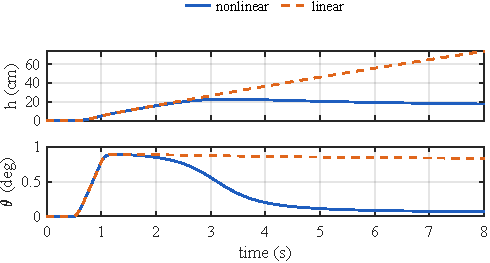
\includegraphics[width=\columnwidth]{fig_openloop}
\caption{Open loop: response to a \SI{1}{\degree} front-foil pulse of
\SI{0.5}{s}. The linear model drifts away; in the nonlinear model the foil nears
the surface and loses lift.}
\label{fig:openloop}
\end{figure}

\subsection{Design criteria}

From these aims we derive the criteria of Table~\ref{tab:req}. R1 covers the
expected speed and payload range. R2 lets the pilot change height in a few
seconds; the overshoot bound keeps a \SI{5}{cm} step within \SI{5}{mm}. R3 is
needed because a speed or mass error changes the lift needed at trim, which acts
on the boat as a constant vertical force. R4 follows from the actuator limits.
R5 bounds the height error so that three standard deviations (\SI{6}{cm}) stay
within \SI{20}{\percent} of the foil submergence and inside the range where the
linear model holds.

\begin{table}[t]
\centering
\caption{Design criteria (nonlinear model, actuator limits, sensor noise)}
\label{tab:req}
\small
\begin{tabular}{@{}lp{6.9cm}@{}}
\toprule
R1 & Closed loop stable for $U\in[6,9]$\,\si{m/s}, $m\in[190,240]$\,\si{kg}. \\
R2 & \SI{5}{cm} height step: \SI{2}{\percent} settling within \SI{2.5}{s}, overshoot below \SI{10}{\percent}. \\
R3 & Zero steady-state error in $h$ and $\theta$ under speed and mass errors. \\
R4 & Foil deflection within the \SI{+3.5}{\degree} upward margin and rate within \SI{20}{\degree/s} in normal operation. \\
R5 & Height error below \SI{2}{cm} rms in the \SI{5}{cm} regular wave and in the mildest irregular sea (S1). \\
\bottomrule
\end{tabular}
\end{table}

%=====================================================================
\section{Controller Design}
\label{sec:design}

\subsection{Reachability, observability and sensors}

The reachability matrix $[B\;AB\;A^2B\;A^3B]$ has rank 4, also with either foil
alone. The observability matrix of $(A,C)$ has rank 4, also with any single
sensor, so rank does not decide which sensors are needed. Robustness does. A
speed or mass error acts as a constant vertical force $b$, which we add to the
observer as a fifth state with $\dot v=\dots+b$. With all three sensors the
augmented pair $(A_e,C_e)$ is observable (rank 5). With only the height sensor
and the gyro it is observable but weakly: the slowest observer pole drops to
about \SI{-0.005}{rad/s}, and in simulation a speed \SI{1}{m/s} too low left the
boat \SI{12.6}{cm} low and pitched \SI{2.4}{\degree} while the estimates read
zero. A force and a pitch offset produce the same bow reading; the AHRS pitch
angle separates them. We therefore use all three sensors; heave and heave rate
remain unmeasured ($n_y=3<n_x=4$).

\subsection{State feedback with integral action}

The control law (Fig.~\ref{fig:loop}) is
\begin{equation}
\tilde{\bm u}=\bm N_u r_f-K(\hat{\bm x}-\bm N_x r_f)-K_i\bm\xi,\quad
\dot{\bm\xi}=\begin{bmatrix}\hat h-r_f\\ y_2\end{bmatrix},
\label{eq:law}
\end{equation}
where $r_f$ is the height command after a first-order prefilter
($t_f=\SI{0.6}{s}$) and $\bm N_x,\bm N_u$ give the steady state for a height
$r$ with level pitch. The integrators act on the \emph{estimated} height and the
\emph{measured} pitch: integrating the raw bow reading would make the boat
follow the water surface. They are frozen while a command saturates
(anti-windup). $K$ and $K_i$ minimise
$J=\int(\bm x_a\T Q\bm x_a+\tilde{\bm u}\T R\tilde{\bm u})\,dt$ for the
augmented model $\bm x_a=[\bm x;\bm\xi]$, which is reachable (rank 6). The
weights follow Bryson's rule \cite{bryson}: \SI{2}{cm} of heave,
\SI{0.5}{m/s} of heave rate, \SI{2}{\degree} of pitch, \SI{10}{\degree/s} of
pitch rate and \SI{3}{\degree} of each foil. The integral weights,
$10/0.02^2$ and $10/(1^\circ)^2$, were tuned. The closed-loop poles are
$-3.32$, $-3.90\pm2.35j$, $-10.8\pm5.6j$ and $-18.5$. The gains are physical:
a height error moves both foils the same way, a pitch error moves them in
opposite directions.

\begin{figure}[t]
\centering
% Control loop. The dashed box is the 50 Hz digital controller, which runs
% either inside the Simulink model or as a separate process over TCP.
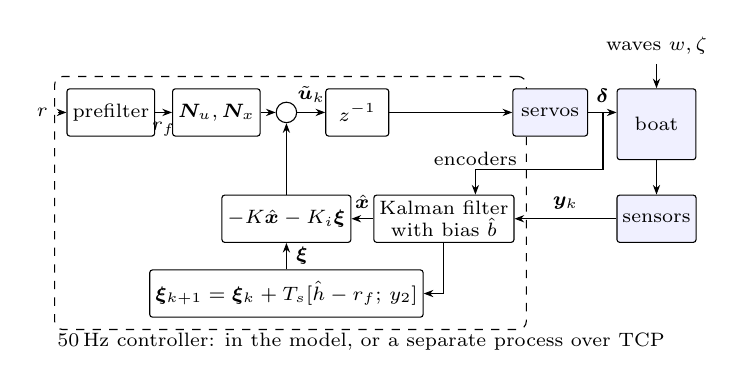
\begin{tikzpicture}[font=\scriptsize, >={Stealth[length=3.5pt]},
  blk/.style={draw, rounded corners=1pt, minimum height=0.6cm, inner sep=2pt, align=center, fill=white},
  phys/.style={blk, fill=blue!6},
  sum/.style={draw, circle, inner sep=0pt, minimum size=0.26cm, fill=white}]
  % top row
  \node (r) at (-0.15,0) {$r$};
  \node[blk, minimum width=0.95cm] (pf) at (0.72,0) {prefilter};
  \node[blk, minimum width=0.9cm]  (ff) at (2.06,0) {$\bm N_u,\bm N_x$};
  \node[sum] (s) at (2.95,0) {};
  \node[blk, minimum width=0.8cm]  (dl) at (3.85,0) {$z^{-1}$};
  \node[phys, minimum width=0.95cm] (act) at (6.3,0) {servos};
  \node[phys, minimum width=1.0cm, minimum height=0.9cm] (boat) at (7.65,-0.15) {boat};
  % feedback rows
  \node[phys, minimum width=1.0cm] (sens) at (7.65,-1.35) {sensors};
  \node[blk, minimum width=1.4cm] (kf) at (4.95,-1.35) {Kalman filter\\with bias $\hat b$};
  \node[blk, minimum width=1.25cm] (lqr) at (2.95,-1.35) {$-K\hat{\bm x}-K_i\bm\xi$};
  \node[blk, minimum width=1.25cm] (int) at (2.95,-2.3) {$\bm\xi_{k+1}=\bm\xi_k+T_s[\hat h-r_f;\,y_2]$};
  % waves
  \node (w) at (7.65,0.85) {waves $w,\zeta$};
  \draw[->] (w) -- (boat);
  % forward path
  \draw[->] (r) -- (pf);
  \draw[->] (pf) -- node[below] {$r_f$} (ff);
  \draw[->] (ff) -- (s);
  \draw[->] (s) -- node[above] {$\tilde{\bm u}_k$} (dl);
  \draw[->] (dl) -- (act);
  \draw[->] (act) -- node[above] {$\bm\delta$} (act -| boat.west);
  % feedback
  \draw[->] (boat) -- (sens);
  \draw[->] (sens) -- node[above] {$\bm y_k$} (kf);
  \draw[->] (6.97,0) -- (6.97,-0.72) -| node[pos=0.62, above] {encoders} ($(kf.north)+(0.4,0)$);
  \draw[->] (kf) -- node[above] {$\hat{\bm x}$} (lqr);
  \draw[->] (lqr) -- (s);
  \draw[->] (kf.south) |- (int.east);
  \draw[->] (int) -- node[right] {$\bm\xi$} (lqr);
  % controller boundary
  \begin{scope}[on background layer]
    \node[draw, dashed, rounded corners=3pt, fit=(pf) (ff) (dl) (kf) (int), inner sep=0.15cm] (box) {};
  \end{scope}
  \node[anchor=north west, inner sep=1pt] at (box.south west) {50\,Hz controller: in the model, or a separate process over TCP};
\end{tikzpicture}

\caption{Control loop. The dashed box runs every \SI{20}{ms}; its command is
applied one sample later. It runs inside the simulation or, in the
software-in-the-loop test, as a separate process.}
\label{fig:loop}
\end{figure}

\subsection{Kalman filter with a force bias}

The observer is a steady-state Kalman filter for the augmented model. The
process noise is the wave velocity entering through $E$ (variance
$0.11^2/2$, correlation time \SI{0.1}{s}) and a random walk on $b$ of intensity
$b_{\mathrm{rate}}^2$, $b_{\mathrm{rate}}=\SI{0.5}{m.s^{-5/2}}$. The decisive
choice is the height noise. The wave surface in $y_1$ has a variance of
$\zeta_a^2/2$ concentrated in a band of about $\Delta f=\SI{0.25}{Hz}$ around the
encounter frequency, so its spectral density there is $\zeta_a^2/(4\Delta f)$,
about 100 times what the same variance spread as white noise would give. Using
this value makes the filter trust the model and the AHRS at wave frequencies.
The resulting observer poles are $-0.66$, $-0.67\pm0.62j$, $-12$ and $-287$:
fast for the measured pitch, slow for the heave and the bias. The observer is
slower than the controller, against the usual rule of thumb; the separation
principle still applies, and the loop of plant, observer and integrators has
exactly the poles of the two designs (difference below $10^{-12}$).
$b_{\mathrm{rate}}$ sets a trade-off: a larger value recovers faster from a
speed change but follows long waves more.

\subsection{Pole placement or Kalman filter}

The usual design rule places the observer poles two to five times faster than
the controller's. Table~\ref{tab:obs} compares three such observers with
the Kalman filter, all with the same digital controller (Section~\ref{sec:dig}):
PP-3x and PP-1x place the five poles at 3 and 1 times the five slowest
controller poles, and PP-KF at the poles of the Kalman filter.

\begin{table}[t]
\centering
\caption{Observer comparison (nonlinear model, \SI{50}{Hz}). Waves: \SI{5}{cm}
step in the regular wave with noise. S2: irregular sea, three seeds. Speed
error: true speed \SI{6}{m/s}, peak height deviation and time to return within
\SI{5}{mm}; with PP-KF the hull touched the water after \SI{4.3}{s}.}
\label{tab:obs}
\small
\setlength{\tabcolsep}{3.5pt}
\begin{tabular}{@{}lccccc@{}}
\toprule
 & \multicolumn{3}{c}{regular wave} & S2 & speed error \\
Observer & $h$ err & $\hat h$ err & rate & $h$ err & peak / return \\
 & (cm rms) & (cm rms) & (\si{\degree/s}) & (cm rms) & \\ \midrule
Kalman & 0.99 & 0.71 & 4.6 & 2.0--2.3 & \SI{15}{cm} / \SI{7.6}{s} \\
PP-3x & 4.28 & 3.35 & 19.2 & 8.9--9.5 & \SI{2.8}{cm} / \SI{0.7}{s} \\
PP-1x & 3.41 & 3.67 & 19.3 & 8.6--10.2 & \SI{4.1}{cm} / \SI{1.2}{s} \\
PP-KF & 2.71 & 0.72 & 18.3 & 2.1--2.2 & diverges \\
\bottomrule
\end{tabular}
\end{table}

\begin{figure}[t]
\centering
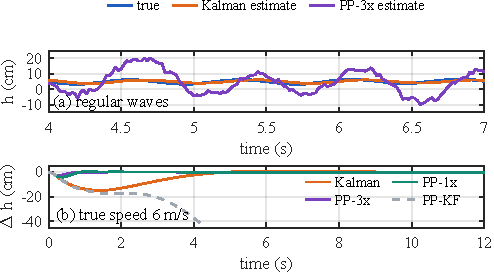
\includegraphics[width=\columnwidth]{fig_observers}
\caption{(a) Heave estimate in the regular wave: the fast pole-placement
observer follows the water surface. (b) Height deviation from the nominal
response when the true speed is \SI{6}{m/s}.}
\label{fig:obs}
\end{figure}

The fast observers limit the deviation after a speed error to a fifth and
recover ten times sooner, but they reconstruct the heave mostly from the bow
reading and so follow the water
surface (Fig.~\ref{fig:obs}a): the height error in waves is four times larger
and the foils run at the \SI{20}{\degree/s} rate limit most of the time,
which violates R4 and R5. PP-KF shows why pole locations are not enough with
three outputs: its poles equal the Kalman filter's, yet the different gain
matrix, i.e.\ different eigenvectors and a different weighting of the sensors,
makes the foils chatter in waves and lets a speed error drive the hull into the
water. The Kalman filter sets the gain from the noise statistics and is the
only one that meets R5 and keeps the foil rate well below its limit; its price
is a slower recovery from model errors.

\subsection{Digital implementation}
\label{sec:dig}

The controller runs at \SI{50}{Hz}. Running the continuous design with a
\SI{20}{ms} Euler step fails: the observer pole at \SI{-287}{rad/s} maps to
$1-287\cdot0.02=-4.74$, outside the unit circle (stability needs
$T_s<\SI{7}{ms}$). We therefore redesign in discrete time \cite{franklin}. The
plant is discretised with a zero-order hold; the LQR is computed with
\texttt{dlqr} on the augmented model with weights $QT_s$, $RT_s$; the Kalman
filter with \texttt{dlqe} in current-estimator form, with the process noise
discretised exactly \cite{vanloan} and the measurement covariance
$R_n/T_s$. The command computed from the samples at $t_k$ is applied at
$t_{k+1}$, and this delay is part of the design model through the extra state
$\tilde{\bm u}_{k-1}$. Each sample the controller executes
\begin{align*}
\hat{\bm x}_{k|k-1}&=A_{de}\hat{\bm x}_{k-1}+B_{de}(\bar{\bm\delta}_k-\bm u_0),\\
\hat{\bm x}_k&=\hat{\bm x}_{k|k-1}+M(\bm y_k-C_e\hat{\bm x}_{k|k-1}),\\
\tilde{\bm u}_k&=\bm N_ur_f-K_d(\hat{\bm x}_k-\bm N_xr_f)-K_{id}\bm\xi_k\\
&\quad-K_u(\tilde{\bm u}_{k-1}-\bm N_ur_f),
\end{align*}
followed by the integrator and prefilter updates, where $\bar{\bm\delta}_k$ is
the mean encoder reading over the last interval. The equivalent poles of the
digital LQR match the continuous ones within \SI{1}{\percent}. Those of the
filter are $-0.67\pm0.62j$, $-1.28$, $-12$ and $-178$; the difference from the
continuous filter is a sampling effect and vanishes as $T_s\to0$.

Table~\ref{tab:rate} repeats the design and the wave test at other rates. The
error grows gradually down to \SI{15}{Hz}. At \SI{10}{Hz} the loop fails although
the design model is stable: the servo lag, which the design model omits, then
destabilises a mode at the Nyquist frequency (\SI{5}{Hz}, $|z|=1.04$). We keep
\SI{50}{Hz}, three times above the slowest acceptable rate; \SI{100}{Hz} would
gain only \SI{0.05}{cm}.

\begin{table}[t]
\centering
\caption{Controller rate: \SI{5}{cm} step in the regular wave with noise,
design redone for each rate}
\label{tab:rate}
\small
\begin{tabular}{@{}lcccccc@{}}
\toprule
Rate (Hz) & 100 & 50 & 25 & 20 & 15 & 10 \\ \midrule
$h$ error (cm rms) & 0.94 & 0.99 & 1.09 & 1.17 & 1.34 & 16.8 \\
$\theta$ (deg rms) & 0.30 & 0.33 & 0.39 & 0.45 & 0.49 & 2.42 \\
\bottomrule
\end{tabular}
\end{table}

\subsection{Closed-loop stability and robustness}

The digital loop with the delay was checked on a grid of
$U\in[5.9,9]$\,\si{m/s} and $m\in[190,240]$\,\si{kg}: the largest closed-loop pole
magnitude is 0.989, so R1 holds.

%=====================================================================
\section{Numerical Validation}
\label{sec:valid}

All tests use the nonlinear model \eqref{eq:vfoil}--\eqref{eq:meas},
integrated with \texttt{ode45} between samples, with sampled noisy sensors,
actuator limits, rate limit and servo lag. The same model built in Simulink
agrees with the MATLAB simulation to \SI{1e-10}{m} in open loop and
\SI{0.33}{mm} in closed loop with waves. The MATLAB and Simulink files that
accompany this paper reproduce every figure and table.

\subsection{Tracking and regular waves}

Fig.~\ref{fig:cl} shows a \SI{5}{cm} step in the regular wave. In calm water the
step settles in \SI{2.16}{s} without overshoot (R2). In waves the height error is
\SI{0.99}{cm} rms and the pitch \SI{0.33}{\degree} rms (R5). The heave estimate
ignores most of the \SI{\pm10}{cm} scatter of the bow reading. The front foil moves by at most
\SI{1.3}{\degree} from trim (R4); its rate is \SI{4.6}{\degree/s} rms and reaches
the \SI{20}{\degree/s} limit only in short peaks.

\begin{figure}[t]
\centering
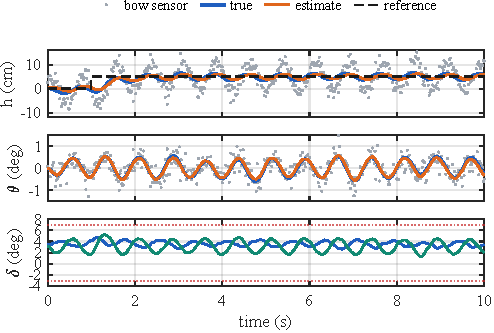
\includegraphics[width=\columnwidth]{fig_closedloop}
\caption{\SI{5}{cm} step in the regular wave with sensor noise: height from the
bow sensor (dots), true and estimated height and pitch, and foil angles.}
\label{fig:cl}
\end{figure}

\subsection{Estimation error}

To check that the estimation error converges, Fig.~\ref{fig:est} starts the
boat \SI{5}{cm} high and \SI{1}{\degree} bow-up while the estimate starts at zero,
in the regular wave with noise. The pitch error falls below \SI{0.1}{\degree}
within \SI{2}{s} and the heave error within about \SI{1.5}{s} to a bounded
oscillation at the encounter frequency, the part of the wave surface the filter
cannot separate from boat motion. After \SI{3}{s} the errors are \SI{0.82}{cm},
\SI{1.7}{cm/s}, \SI{0.05}{\degree} and \SI{0.21}{\degree/s} rms for $h$, $v$,
$\theta$ and $q$.

\begin{figure}[t]
\centering
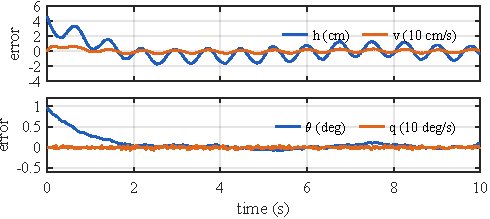
\includegraphics[width=\columnwidth]{fig_estimation}
\caption{Estimation errors from a wrong initial estimate (boat \SI{5}{cm} high,
\SI{1}{\degree} bow-up), regular wave with noise.}
\label{fig:est}
\end{figure}

\subsection{Model uncertainty}

Fig.~\ref{fig:robust} repeats the calm-water step with the true speed or mass
away from the design values. The bias estimate converges to the force each
error causes and the integrators remove the remaining error: height and pitch
return to their targets in every case (R3). The worst case, a speed
\SI{1}{m/s} too low, gives a \SI{15}{cm} transient that is back within
\SI{5}{mm} after \SI{7.6}{s}. This is the cost of the slow observer
(Table~\ref{tab:obs}); scheduling the trim angles on the measured speed would
remove most of it.

\begin{figure}[t]
\centering
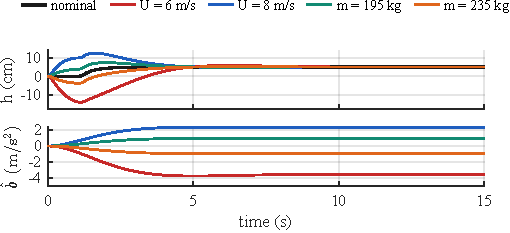
\includegraphics[width=\columnwidth]{fig_robust}
\caption{\SI{5}{cm} step with speed and mass errors (calm water) and the
estimated force bias $\hat b$.}
\label{fig:robust}
\end{figure}

\subsection{Irregular seas}

Table~\ref{tab:irr} gives the results in three JONSWAP sea states, five random
seas each. In S1 the error matches the regular wave (R5). It then grows faster
than the wave height, because the longer waves of S2 and S3 are met at lower
frequencies, where the filter cannot tell the water surface from slow boat
motion. Pitch, which is measured, stays below \SI{0.4}{\degree} rms. In S3 the
front foil reaches its limit for up to \SI{0.5}{\percent} of the time.
Fig.~\ref{fig:irr} shows S2: the estimate follows the slow part of the boat
motion but not the \SI{\pm10}{cm} water surface, and the front foil uses at
most about two thirds of its upward margin.

\begin{figure}[t]
\centering
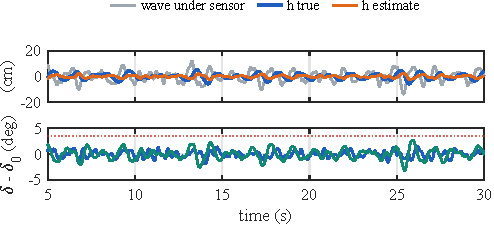
\includegraphics[width=\columnwidth]{fig_irregular}
\caption{Sea state S2 ($H_s=\SI{0.15}{m}$, $T_p=\SI{3}{s}$): water surface
under the sensor, true and estimated heave, and foil deflections from trim.}
\label{fig:irr}
\end{figure}

\begin{table}[t]
\centering
\caption{Irregular head seas: range over five seas (after \SI{5}{s})}
\label{tab:irr}
\small
\setlength{\tabcolsep}{3.5pt}
\begin{tabular}{@{}lcccccc@{}}
\toprule
Sea & $H_s$ & $T_p$ & $h$ err rms & $\theta$ rms & foil peak & sat. \\
 & (m) & (s) & (cm) & (deg) & (deg) & (\%) \\ \midrule
S1 & 0.10 & 2.3 & 0.72--0.81 & 0.20--0.21 & 1.5--2.3 & 0 \\
S2 & 0.15 & 3.0 & 1.8--2.2 & 0.25--0.28 & 1.8--2.5 & 0 \\
S3 & 0.25 & 3.5 & 3.6--4.9 & 0.34--0.40 & 2.6--4.7 & 0--0.5 \\
\bottomrule
\end{tabular}
\end{table}

\subsection{Software in the loop}

To test the controller as it would run on the boat's computer, we moved it into
a separate MATLAB process. The Simulink model of the boat sends the sensor and
encoder readings every \SI{20}{ms} over TCP and applies the reply at the next
sample, which is the delay of the design; the controller never sees the true
state. Two modes are used. In \emph{lockstep} the model waits for each reply;
the trajectory is then identical to the in-model controller (difference
exactly zero), which shows that the split changes nothing. In \emph{real time}
the model is paced to the wall clock and holds the last command when a reply
is late. A round trip takes \SI{0.24}{ms} (median) and the control algorithm
\SI{0.1}{ms}, and the simulation keeps to the clock to within \SI{0.6}{ms} per
step.

\begin{figure}[t]
\centering
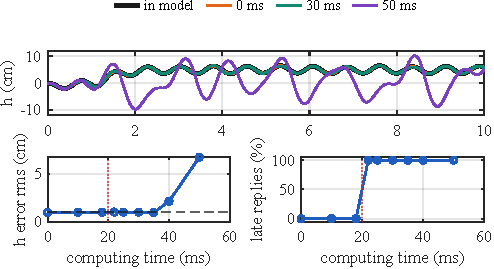
\includegraphics[width=\columnwidth]{fig_sil}
\caption{Controller as a separate real-time process with added computing time:
height for three cases, height error and share of late replies.}
\label{fig:sil}
\end{figure}

We then slowed the controller down (Fig.~\ref{fig:sil}). Up to \SI{18}{ms} of
computing time nothing changes. From \SI{22}{ms} to \SI{35}{ms} every reply is
one sample late, yet the height error stays at 0.94--\SI{0.99}{cm}. At
\SI{40}{ms} it doubles (\SI{2.1}{cm}) and at \SI{50}{ms} the boat oscillates by
\SI{\pm10}{cm}. A linear analysis with $n$ extra samples of delay agrees: the
damping ratio of a \SI{2}{Hz} mode falls from 0.62 to 0.32, 0.11 and $-0.03$
for $n=0$ to 3. Random computing times of 10 to \SI{30}{ms} made \SI{80}{\percent}
of replies late, because a late reply delays the next one, with an error of
\SI{1.00}{cm}. The controller must therefore finish within one period, with one
sample of tolerance; its actual time on the boat's microcontroller should be
measured. Both processes ran on one computer, so network delays and clock drift
of a real system are not represented.

\begin{table}[t]
\centering
\caption{Design criteria and results}
\label{tab:summary}
\small
\begin{tabular}{@{}lp{5.4cm}c@{}}
\toprule
 & Result & Met \\ \midrule
R1 & largest pole magnitude 0.989 over the grid & yes \\
R2 & settling \SI{2.16}{s}, no overshoot & yes \\
R3 & zero error for $U=6,8$\,\si{m/s}, $m=195,235$\,\si{kg} & yes \\
R4 & deflection \SI{1.3}{\degree}; rate limit reached in short peaks & partly \\
R5 & 0.99\,cm (regular), 0.72--0.81\,cm (S1) & yes \\
\bottomrule
\end{tabular}
\end{table}

%=====================================================================
\section{Conclusions}
\label{sec:concl}

A fully submerged hydrofoil boat is open-loop unstable in heave, and its only
height sensor sees the waves. An LQR with integral action on the estimated
height and measured pitch, combined with a Kalman filter that models the water
surface as narrow-band noise and estimates a force bias, meets the design
criteria on the nonlinear model at \SI{50}{Hz} with a computation delay
(Table~\ref{tab:summary}); the rate limit is touched only in short peaks.
Pole-placement observers designed by the usual rule recover faster from model
errors but follow the water surface and saturate the actuators, and placing
the poles where the Kalman filter puts them is not enough. Run as a separate
real-time process, the controller reproduces the in-model results and tolerates
one sample of extra delay. Future work: scheduling the trim and gains on the
measured speed, which would shorten the \SI{8}{s} recovery from speed errors;
a second height sensor or an accelerometer for long waves; and tests on the
boat's microcontroller.

\begin{thebibliography}{10}
\bibitem{belime} B.~J.~Belime, ``An hydrofoil control system for the SR02
vessel in the scope of the T\'ecnico Solar Boat Project,'' M.Sc.\ thesis,
Instituto Superior T\'ecnico, Univ.\ Lisboa, Lisbon, Portugal, 2020.
\bibitem{marrewijk} G.~P.~van Marrewijk and J.~K.~Schonebaum, ``An
experimentally validated dynamical model of a single-track hydrofoil boat,''
TU Delft Solar Boat Team, Delft Univ.\ Technol., Delft, The Netherlands, 2017.
\bibitem{faltinsen} O.~M.~Faltinsen, \emph{Hydrodynamics of High-Speed Marine
Vehicles}. Cambridge, U.K.: Cambridge Univ.\ Press, 2005.
\bibitem{renyang} J.~Ren and Y.~Yang, ``Fuzzy gain scheduling attitude control
for hydrofoil catamaran,'' in \emph{Proc.\ Amer.\ Control Conf.}, Boston, MA,
USA, 2004, pp.~1103--1108.
\bibitem{liu} H.~Liu, Y.~Fu, and B.~Li, ``Study of the LQRY-SMC control method
for the longitudinal motion of fully submerged hydrofoil crafts,'' \emph{J.\
Mar.\ Sci.\ Eng.}, vol.~10, no.~10, Art.\ no.~1390, 2022.
\bibitem{jonswap} K.~Hasselmann \emph{et~al.}, ``Measurements of wind-wave
growth and swell decay during the Joint North Sea Wave Project (JONSWAP),''
\emph{Erg\"anzungsheft zur Deutschen Hydrographischen Zeitschrift, Reihe A},
no.~12, 1973.
\bibitem{bryson} A.~E.~Bryson and Y.-C.~Ho, \emph{Applied Optimal Control}.
Washington, DC, USA: Hemisphere, 1975.
\bibitem{franklin} G.~F.~Franklin, J.~D.~Powell, and M.~L.~Workman,
\emph{Digital Control of Dynamic Systems}, 3rd~ed. Menlo Park, CA, USA:
Addison-Wesley, 1998.
\bibitem{vanloan} C.~F.~Van Loan, ``Computing integrals involving the matrix
exponential,'' \emph{IEEE Trans.\ Autom.\ Control}, vol.~23, no.~3,
pp.~395--404, Jun.\ 1978.
\end{thebibliography}

\end{document}
